\documentclass[tikz]{standalone}

\pagestyle{empty}


\usepackage{amsmath}
\usepackage{tikz}
\usepackage{graphicx}
\usetikzlibrary{positioning,calc,fit,decorations.pathreplacing,arrows,positioning,backgrounds}

% Font settings:
\renewcommand{\familydefault}{\sfdefault}
\usepackage{pxfonts}
\newcommand{\figf}{\sffamily\bfseries\small} %Defines the font used for the labelling of figure panels.


% Color settings:
%\definecolor{hivc}{cmyk}{0,0.80,0.83,0.13}                %\definecolor{hivc}{HTML}{DE2D26}
\definecolor{hivc}{RGB}{24,116,205}
\definecolor{selfc}{cmyk}{0,0,0,0.6}                      %\colorlet{selfc}{gray!80!white}
\definecolor{Rblue}{RGB}{100,149,237}


\begin{document}

\begin{tikzpicture}[anchor=north west]


\begin{scope}
	\node[anchor = north west] at (0,0) {
		\includegraphics{../plots/SF5panel-speed.pdf}
	};
	\node[anchor = north west] at (0,0) {\figf A};		
\end{scope}

\begin{scope}[yshift=-5.8cm]
	\node[anchor = north west] at (0,0) {
		\includegraphics{../plots/SF5panel-persistence.pdf}
	};
	\node[anchor = north west] at (0,0) {\figf B};		
\end{scope}

\begin{scope}[yshift=-11.6cm]

	\node[anchor = north west] at (0,-0.3) {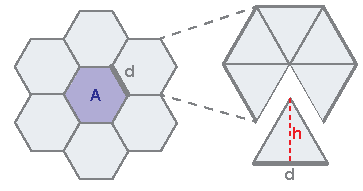
\includegraphics{../cartoons/geometry.pdf}};

	\node[anchor = north west] (eq1) at (7.5,-0.3) {$h^2 + (\frac{d}{2})^2 = d^2$};
	\node[anchor = north west, below = 0mm of eq1.south] (eq2) {$h = \frac{d}{2}\sqrt{3}$};
	\node[anchor = north west, below = 0mm of eq2.south] (eq3) {$A = 6 \cdot (\frac{1}{2}dh) = \frac{3}{2}d^2\sqrt{3}$};
	\node[anchor = north west, below = 0mm of eq3.south] (eq4) {$d = \sqrt{\frac{A}{\frac{3}{2}\sqrt{3}}} = \sqrt{ \frac{2A}{3\sqrt{3}} }$};

	\node at (0,0) {\figf C};
\end{scope}


\end{tikzpicture}


\end{document}